\documentclass[10pt,a4paper]{article}
\usepackage[margin=2.2cm]{geometry}
\usepackage{amsmath,amssymb,bm,booktabs,graphicx,siunitx,hyperref}
\newcommand{\Cof}{\operatorname{cof}}
\newcommand{\tr}{\operatorname{tr}}
\newcommand{\R}{\mathbb{R}}
\newcommand{\FreeEnergyError}{2.077\%}
\newcommand{\FreeStressError}{4.551\%}
\newcommand{\FreeSxxError}{4.062\%}
\newcommand{\FreeSyyError}{5.001\%}
\newcommand{\FreeSxyError}{9.477\%}
\newcommand{\MetricEnergyError}{0.061\%}
\newcommand{\MetricStressError}{0.114\%}
\newcommand{\MetricSxxError}{0.130\%}
\newcommand{\MetricSyyError}{0.095\%}
\newcommand{\MetricSxyError}{0.902\%}
\newcommand{\PolyEnergyError}{1.848\%}
\newcommand{\PolyStressError}{2.643\%}
\newcommand{\PolySxxError}{2.064\%}
\newcommand{\PolySyyError}{3.125\%}
\newcommand{\PolySxyError}{9.375\%}
\newcommand{\HPROMEnergyError}{0.000\%}
\newcommand{\HPROMStressError}{0.118\%}
\newcommand{\HPROMSxxError}{0.109\%}
\newcommand{\HPROMSyyError}{0.117\%}
\newcommand{\HPROMSxyError}{13.338\%}
\newcommand{\RankOneCurvature}{4.609e-01\,\mathrm{GPa}}
\newcommand{\BarrierCoefficient}{3.0728e-01}
\newcommand{\QuadraticCoefficient}{3.1221e-05}
\newcommand{\SampledMinimumEnergy}{5.888e-04\,\mathrm{GPa}}
\newcommand{\MetricTangentDistance}{0.222\%}
\newcommand{\MetricIdentityDistance}{0.374\%}
\newcommand{\FomStageTenTangentMinimum}{-0.0648\,\mathrm{GPa}}


\title{Energy-based neural constitutive surrogates for the nonlinear hyperelastic RVE\\
\large Anisotropy, local tangent scaling, and a constructive polyconvex PANN}
\author{}
\date{\today}

\begin{document}
\maketitle

\begin{abstract}
This memorandum documents a controlled constitutive-learning study for the
two-dimensional nonlinear hyperelastic representative volume element (RVE).
Three models are considered: a flexible energy PANN in material components of
$C$, the same type of PANN in locally isotropised tangent coordinates, and a
polyconvex PANN.  The last is a new constructive model: it is objective,
stress-free in the reference configuration, anisotropic without imposing
$D_4$, energy--stress consistent, polyconvex in $(F,\Cof F,\det F)$, and has
a volumetric barrier.  All stresses are obtained by differentiation of the
same scalar energy.  The three models are trained from Stage--1 trajectories
only and evaluated on Stage--10.
\end{abstract}

\section{Purpose and modelling decision}
\label{sec:purpose}
The goal is not to learn three stress-time curves separately.  The target is
one macroscopic stored-energy density $W$ of the RVE.  Once $W$ is known, the
second Piola stress follows by differentiation.  This makes the energy and
the stress mutually consistent by construction.

The RVE is treated here as a \emph{general anisotropic} material.  In
particular, no square symmetry is assumed.  A $D_4$ model would require the
additional identity
\begin{equation}
 W(C_{11},C_{22},C_{12})=W(C_{22},C_{11},-C_{12}),
 \label{eq:d4}
\end{equation}
which is not used below.  This is a modelling decision, not a statement that
the square-shaped numerical cell makes the effective material isotropic.

\section{Kinematics, stress convention, and objectivity}
\label{sec:kinematics}
Let
\begin{equation}
 C=F^TF,\qquad E=\frac12(C-I),\qquad J=\det F=\sqrt{\det C}>0.
 \label{eq:kinematics}
\end{equation}
The database and all neural models use the engineering-shear coordinate
\begin{equation}
 \bm e=\begin{bmatrix}E_{11}\\E_{22}\\\gamma_{12}\end{bmatrix},
 \qquad \gamma_{12}=2E_{12}.
 \label{eq:e-coordinate}
\end{equation}
The work identity is therefore
\begin{equation}
 dW=S_{11}\,dE_{11}+S_{22}\,dE_{22}+S_{12}\,d\gamma_{12},\qquad
 \frac{\partial W}{\partial\bm e}
 =\begin{bmatrix}S_{11}\\S_{22}\\S_{12}\end{bmatrix}.
 \label{eq:stress}
\end{equation}
Equation~\eqref{eq:stress} is crucial: the derivative returns precisely the
second Piola components stored in the direct FOM data; there is no factor-two
ambiguity in the shear component and no independently trained stress network.

Objectivity concerns a rotation of the \emph{current} spatial observer.  For
every proper orthogonal $Q$,
\begin{equation}
 F\mapsto QF\quad\Longrightarrow\quad (QF)^T(QF)=C.
\end{equation}
Consequently, a scalar model built from $C$ (or from the objective minor
norms used in Section~\ref{sec:polyconvex}) satisfies
$W(QF)=W(F)$.  This is different from material symmetry: material symmetry
would rotate the RVE relative to its fixed material axes and is not imposed.

\section{Anisotropic representation}
\label{sec:anisotropy}
Let $a_0$ and $b_0$ be two physical directions attached to the reference RVE.
The independent material contractions in two dimensions are
\begin{equation}
 c_{aa}=a_0\cdot Ca_0,\qquad
 c_{bb}=b_0\cdot Cb_0,\qquad
 c_{ab}=a_0\cdot Cb_0.
 \label{eq:structural-c}
\end{equation}
In the stored RVE coordinates they are $C_{11}$, $C_{22}$, and $C_{12}$.
There are only three independent components of a symmetric $2\times2$ tensor;
``six invariants'' is the corresponding count in three dimensions.  We also
pass $J$ explicitly, although it is redundant through
$J^2=c_{aa}c_{bb}-c_{ab}^2$.  It separates the volumetric state visibly from
the other features.

Under a relabelling of reference axes, $C$, $a_0$, and $b_0$ must be
transformed together.  The three numbers in \eqref{eq:structural-c} are then
unchanged.  This is coordinate covariance, not an extra material symmetry.

\section{Two flexible energy PANNs}
\label{sec:flexible}
\subsection{C-PANN}
The accuracy-oriented reference model is a smooth Softplus MLP
$\widehat W_\theta$ of
\begin{equation}
 \bm z_C=[c_{aa}-1,\ c_{bb}-1,\ c_{ab},\ J-1]^T.
\end{equation}
It is made reference-consistent using the affine correction
\begin{equation}
 W_C(\bm e)=\widehat W_\theta(\bm z_C(\bm e))-
 \widehat W_\theta(\bm z_C(\bm0))-
 \left.\frac{\partial\widehat W_\theta}{\partial\bm e}\right|_{\bm0}\!\cdot\bm e.
 \label{eq:c-pann}
\end{equation}
Thus $W_C(\bm0)=0$ and $\partial W_C/\partial\bm e|_{\bm0}=\bm0$, up to
floating-point roundoff.  This correction is legitimate for a flexible PANN,
but it would generally destroy a polyconvexity certificate.  Hence this model
makes \emph{no} convexity or polyconvexity claim.

\subsection{PANN-T: local anisotropic-to-isotropic tangent scaling}
\label{sec:metric}
The second flexible model tests the idea in the anisotropic mixed-formulation
paper of Rossi, Zorrilla, and Codina~\cite{Rossi2021}.  At the reference
state, the FOM finite-difference tangent is
\begin{equation}
 D_0=\left.\frac{\partial\bm S}{\partial\bm e}\right|_{\bm0}.
\end{equation}
In the coordinates \eqref{eq:e-coordinate}, the closest isotropic tangent
that preserves the uniform-dilation modulus is
\begin{equation}
 \widehat D=
 \begin{bmatrix}
 \lambda+2\mu&\lambda&0\\
 \lambda&\lambda+2\mu&0\\
 0&0&\mu
 \end{bmatrix},\quad
 \kappa=\frac{D_{00}+2D_{01}+D_{11}}{4},\quad
 \mu=\frac{D_{00}-2D_{01}+D_{11}+D_{22}}{5},\quad \lambda=\kappa-\mu.
 \label{eq:closest-isotropic}
\end{equation}
For positive definite $D_0$ and $\widehat D$, define
\begin{equation}
 T=\widehat D^{-1/2}D_0^{1/2},\qquad D_0=T^T\widehat D T.
 \label{eq:metric-map}
\end{equation}
PANN-T uses $[(T\bm e)^T/\varepsilon_\mathrm{scale},J-1]^T$ as the MLP
input and applies the same reference correction as \eqref{eq:c-pann}.
Numerically, $\|D_0-\widehat D\|_F/\|D_0\|_F=\MetricTangentDistance$ and
$\|T-I\|_F/\|I\|_F=\MetricIdentityDistance$.  Thus it is an intentionally
small, local conditioning transformation for this RVE.  It does not make the
nonlinear material isotropic, and it does not imply convexity or
polyconvexity.

\section{Constructive anisotropic polyconvex PANN}
\label{sec:polyconvex}
Polyconvexity is a condition on the deformation gradient:
\begin{equation}
 W(F)=G(F,\Cof F,J),\qquad G\ \text{convex in }(F,\Cof F,J).
 \label{eq:poly-definition}
\end{equation}
It is \emph{not} synonymous with convexity in $E$ or with a positive definite
$\partial\bm S/\partial\bm e$.

For each $k=1,2,3$, choose three unit structural directions $d_{ki}$ and
positive weights $w_{ki}$ satisfying
\begin{equation}
 \sum_{i=1}^{3}w_{ki}\,d_{ki}\otimes d_{ki}=I.
 \label{eq:balanced-directions}
\end{equation}
The three direction systems are
\begin{align*}
 &(0^\circ,50^\circ,130^\circ),\qquad
 (20^\circ,83^\circ,151^\circ),\qquad
 (12^\circ,76^\circ,143^\circ),
\end{align*}
with the positive weights recorded in the reproducibility file.  They have no
$90^\circ$-rotation closure and no $D_4$ average is taken.  From them we form
\begin{align}
 I_1&=\tr C=|F|^2,\nonumber\\
 Q_{k,p}^F&=\sum_{i=1}^3 w_{ki}\,(d_{ki}\cdot Cd_{ki})^p
       =\sum_{i=1}^3 w_{ki}|Fd_{ki}|^{2p},\qquad p=2,3,\nonumber\\
 Q_{k,p}^H&=\sum_{i=1}^3 w_{ki}\,(d_{ki}\cdot\Cof(C)d_{ki})^p
       =\sum_{i=1}^3 w_{ki}|\Cof(F)d_{ki}|^{2p},\qquad p=2,3.
 \label{eq:qfeatures}
\end{align}
The evaluated features are
\begin{equation}
 \bm z_{\rm pc}=(I_1,\{Q_{k,2}^F,Q_{k,3}^F,Q_{k,2}^H,Q_{k,3}^H\}_{k=1}^3,J,J^2).
\end{equation}
Let $\Phi_\theta$ be an input-convex neural network (ICNN) whose input and
hidden-to-hidden weights are non-negative and whose activations are Softplus.
It is then convex and coordinate-wise non-decreasing in $\bm z_{\rm pc}$.
The energy is
\begin{equation}
 W_{\rm pc}(F)=\Phi_\theta(\bm z_{\rm pc})-
 \Phi_\theta(\bm z_{\rm pc}(I))-r\log J+
 \frac{\beta}{2}(J-1)^2,\qquad r,\beta>0.
 \label{eq:pc-energy}
\end{equation}

The sixth-power terms are not cosmetic.  In two dimensions, a balanced
quartic aggregate by itself obeys an accidental $90^\circ$ identity:
if $t_i=d_i\cdot Cd_i$, then the rotated values are
$\tr(C)-t_i$ and the balance relation makes $\sum_iw_i(\tr(C)-t_i)^2=
\sum_iw_it_i^2$.  The cubic aggregate $\sum_iw_it_i^3$ does not obey this
identity in general.  It therefore supplies anisotropic information while its
first derivative at $C=I$ remains isotropic.

\paragraph{Why this is polyconvex.}
For a fixed $d$, $|Fd|^2$ is convex in $F$ and the maps $x\mapsto x^p$ for
$p=2,3$ are convex and increasing for $x\geq0$; hence $|Fd|^{2p}$ is convex
in $F$.  Exactly the same argument holds for $|\Cof(F)d|^{2p}$ as a function
of the cofactor minor.  Positive sums, $I_1$, $J$, and $J^2$ are convex functions of
the corresponding minor variables on $J>0$.  The monotone convex-composition
rule therefore makes the ICNN term convex in $(F,\Cof F,J)$.  Finally,
$-r\log J$ and $\beta(J-1)^2/2$ are convex in $J>0$.  This proves
\eqref{eq:poly-definition}; it is a construction proof, not a numerical
penalty in the loss.

\paragraph{Why the reference stress vanishes without breaking the proof.}
At $C=I$, relation~\eqref{eq:balanced-directions} makes the first derivative
of each $Q_{k,p}^F$ and $Q_{k,p}^H$ isotropic.  The same is true of $I_1$, $J$, and
$J^2$.  Thus the ICNN has a reference derivative of the form $(p,p,0)$ in
the coordinate \eqref{eq:e-coordinate}.  We set
\begin{equation}
 r=p=\frac12\left.
 \left(\frac{\partial\Phi_\theta}{\partial E_{11}}+
       \frac{\partial\Phi_\theta}{\partial E_{22}}\right)\right|_{E=0}.
 \label{eq:pressure-cancellation}
\end{equation}
Since $\partial\log J/\partial\bm e|_{0}=(1,1,0)$, the logarithmic term
cancels this pressure.  Equation~\eqref{eq:pc-energy} consequently gives
$W_{\rm pc}(I)=0$ and $\bm S(I)=\bm0$, while retaining polyconvexity.
Moreover, it diverges as $J\to0^+$ and has positive quadratic growth as
$J\to\infty$.

\section{Training protocol and what is not imposed}
\label{sec:training}
All models minimize a combined relative squared-error loss on direct FOM
energy and direct FOM second Piola stress:
\begin{equation}
 \mathcal L=0.65\,\mathcal L_W+0.35\,\mathcal L_S+0.65\,\mathcal L_{S,\rm comp},
 \label{eq:loss}
\end{equation}
where $\mathcal L_W$ and $\mathcal L_S$ normalize the mean squared energy and
all-component stress errors by their respective mean squared targets, and
$\mathcal L_{S,\rm comp}$ is the equally weighted mean of the three
componentwise normalized stress errors.  In every term the predicted stress
is the derivative in \eqref{eq:stress} of the predicted energy.

All three final models use all 109\,460 saved states of Stage--1 trajectories
1--10.  The certified ICNN is trained in CPU float64 because its
energy--stress loss differentiates the energy twice.  No training script opens
Stage--10.

We deliberately do not impose
\begin{equation}
 \frac{\partial\bm S}{\partial\bm e}\succ0.
 \label{eq:not-spd}
\end{equation}
The independent FOM tangent audit gives a minimum eigenvalue of
$\FomStageTenTangentMinimum$ on a Stage--10 state.  Thus a global version of
\eqref{eq:not-spd} would contradict the FOM response.  Polyconvexity is the
relevant stronger-in-$F$ construction for the third model, but it does not
require a positive strain Hessian.

\section{Held-out Stage--10 assessment}
\label{sec:results}
Table~\ref{tab:results} reports relative $L^2$ errors against the direct FOM
labels.  The direct HPROM--ANN row is a compatible reconstruction of energy
and the same second Piola stress at its stored displacement state; it is not a
separately retrained comparison.

\begin{table}[h]
\centering
\caption{Stage--10 relative $L^2$ errors against direct FOM labels.}
\label{tab:results}
\begin{tabular}{lrrrrr}
\toprule
Model & $W$ & $S$ & $S_{11}$ & $S_{22}$ & $S_{12}$\\
\midrule
Flexible C-PANN & \FreeEnergyError & \FreeStressError & \FreeSxxError & \FreeSyyError & \FreeSxyError\\
PANN-T (local tangent metric) & \MetricEnergyError & \MetricStressError & \MetricSxxError & \MetricSyyError & \MetricSxyError\\
Certified polyconvex PANN & \PolyEnergyError & \PolyStressError & \PolySxxError & \PolySyyError & \PolySxyError\\
Direct HPROM--ANN reconstruction & \HPROMEnergyError & \HPROMStressError & \HPROMSxxError & \HPROMSyyError & \HPROMSxyError\\
\bottomrule
\end{tabular}
\end{table}

\begin{figure}[h]
\centering
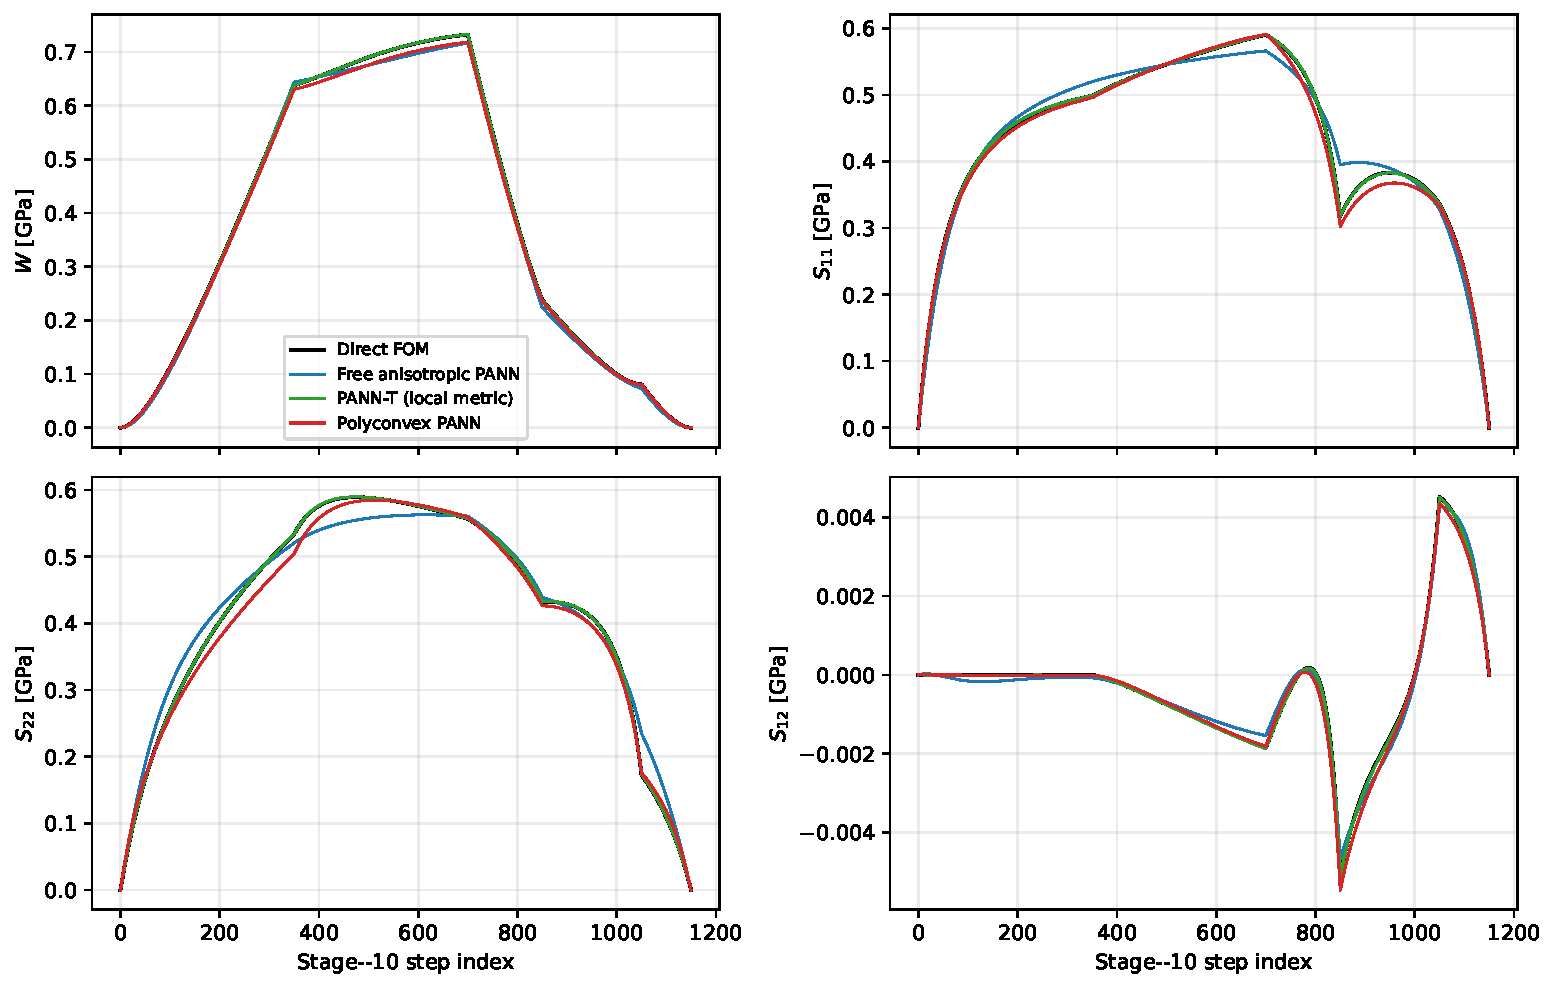
\includegraphics[width=.97\linewidth]{anisotropic_stage10_comparison.pdf}
\caption{Held-out energy and energy-conjugate second Piola components along
Stage--10.  Every PANN stress shown here is differentiated from the displayed
PANN energy.}
\label{fig:stage10}
\end{figure}

The evaluator additionally verifies the reference conditions, objectivity
under $F\mapsto QF$, the absence of an imposed $D_4$ average, and (for the
certified model) numerical rank-one curvature samples.  The smallest sampled
rank-one second derivative is $\RankOneCurvature$.  This sample is not the
proof---the proof is the construction above---but it is a useful attempt to
falsify an implementation error.  The learned volumetric coefficients are
$r=\BarrierCoefficient$ and $\beta=\QuadraticCoefficient$ in normalized
energy units.  A separate broad positive-definite sampling audit found a
minimum energy of $\SampledMinimumEnergy$; this is a useful physical check,
not a proof of global non-negativity.

\begin{figure}[h]
\centering
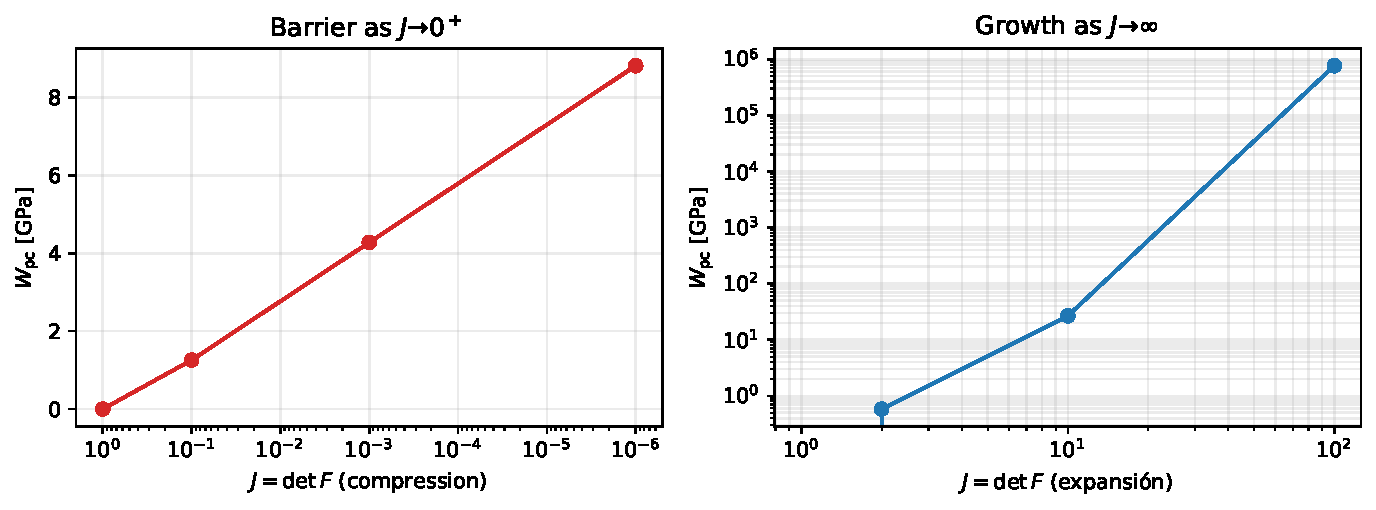
\includegraphics[width=.84\linewidth]{anisotropic_polyconvex_volumetric.pdf}
\caption{Volumetric response of the certified PANN: the logarithmic barrier
acts as $J\to0^+$ and the positive quadratic term supplies growth at large
$J$.}
\label{fig:volumetric}
\end{figure}

\section{Conclusions and recommended use}
The three models answer three distinct questions and should not be presented
as interchangeable black boxes.  The C-PANN is the flexible accuracy
baseline.  PANN-T tests a principled local tangent scaling; it changes the
conditioning, not the physical symmetry class or the global mathematics.  The
third model is the mathematically strongest candidate: its objectivity,
reference state, energy--stress consistency, anisotropic structural response,
polyconvexity, and volumetric barrier are architectural properties.  Its
prediction gap, if present in Table~\ref{tab:results}, is the honest cost of
those restrictions rather than a guarantee silently omitted from the model.

\begin{thebibliography}{9}
\bibitem{Ball1977}
J.~M. Ball. Convexity conditions and existence theorems in nonlinear
elasticity. \emph{Archive for Rational Mechanics and Analysis}, 63:337--403,
1977.
\bibitem{Amos2017}
B. Amos, L. Xu, and J.~Z. Kolter. Input convex neural networks. In
\emph{Proceedings of the 34th International Conference on Machine Learning},
2017.
\bibitem{Ciarlet1988}
P.~G. Ciarlet. \emph{Mathematical Elasticity, Volume I: Three-Dimensional
Elasticity}. North-Holland, 1988.
\bibitem{Rossi2021}
R. Rossi, R. Zorrilla, and R. Codina. A stabilised displacement--volumetric
strain formulation for nearly incompressible and anisotropic materials.
\emph{Computer Methods in Applied Mechanics and Engineering}, 377:113701,
2021. \url{https://doi.org/10.1016/j.cma.2021.113701}.
\end{thebibliography}

\end{document}
